\documentclass[aspectratio=169,10pt]{beamer}

\usepackage[utf8]{inputenc}
\usepackage[T5]{fontenc}
\usepackage[english,vietnamese]{babel}
\usepackage{mathptmx}
\usepackage{array}
\usepackage{booktabs}
\usepackage{graphicx}
\usepackage{tikz}
\usetikzlibrary{arrows.meta,positioning,fit,shapes.geometric}

\AtBeginDocument{\selectlanguage{english}}
\usetheme{default}
\usefonttheme{professionalfonts}
\setbeamertemplate{navigation symbols}{}
\graphicspath{{assets/}{assets/screenshots/}{assets/drawio/}}

\definecolor{EcoparkGreen}{HTML}{0F7B55}
\definecolor{EcoparkTeal}{HTML}{0891B2}
\definecolor{EcoparkAmber}{HTML}{B7791F}
\definecolor{SoftGreen}{HTML}{E8F7EF}
\definecolor{Ink}{HTML}{12201A}
\definecolor{EbpDeep}{HTML}{062E22}
\definecolor{EbpGreen}{HTML}{0F7B55}
\definecolor{EbpTeal}{HTML}{0891B2}
\definecolor{EbpAmber}{HTML}{B7791F}
\definecolor{EbpCanvas}{HTML}{F4FAF7}
\definecolor{EbpPanel}{HTML}{FFFFFF}
\definecolor{EbpBorder}{HTML}{BFDCCF}
\definecolor{EbpMuted}{HTML}{61746A}
\definecolor{EbpLogoGreen}{HTML}{25AD73}
\definecolor{EbpLogoTeal}{HTML}{0B6685}
\setbeamercolor{normal text}{fg=Ink,bg=EbpCanvas}
\setbeamercolor{structure}{fg=EbpGreen}
\setbeamercolor{frametitle}{fg=white,bg=EbpDeep}
\setbeamercolor{block title}{fg=white,bg=EbpGreen}
\setbeamercolor{block body}{fg=Ink,bg=white}
\setbeamertemplate{itemize item}{\raisebox{0.18ex}{\tikz\fill[EbpGreen] (0,0) rectangle (0.08,0.08);}}
\setbeamertemplate{itemize subitem}{\raisebox{0.22ex}{\tikz\fill[EbpTeal] (0,0) circle (0.035);}}
\setbeamertemplate{background canvas}{%
  \begin{tikzpicture}[remember picture,overlay]
    \fill[EbpCanvas] (current page.south west) rectangle (current page.north east);
    \draw[EbpBorder,opacity=0.18] (current page.south west) grid[step=0.62cm] (current page.north east);
  \end{tikzpicture}%
}
\newcommand{\EbpLogo}{%
  \tikz[baseline=-0.56ex,x=0.0156cm,y=0.0156cm]{
    \shade[rounded corners=3.5pt,left color=EbpLogoGreen,right color=EbpLogoTeal] (0,0) rectangle (46,46);
    \draw[white,opacity=0.22,line width=0.35pt,rounded corners=3.5pt] (0.55,0.55) rectangle (45.45,45.45);
    \draw[white,line width=0.9pt,line cap=round,line join=round]
      (29.5,17.5) circle (3.5);
    \draw[white,line width=0.9pt,line cap=round,line join=round]
      (16.5,17.5) circle (3.5);
    \draw[white,line width=0.9pt,line cap=round,line join=round]
      (23,17.5) -- (23,21) -- (20,24) -- (24,27) -- (26,24) -- (28,24);
    \draw[white,line width=0.9pt,line cap=round,line join=round] (26,30) circle (1);
  }%
}
\newcommand{\slidecaption}[1]{%
  \vspace{1.5mm}
  {\scriptsize\bfseries\color{EbpDeep}#1}
}
\setbeamertemplate{frametitle}{%
  \nointerlineskip
  \begin{beamercolorbox}[wd=\paperwidth,ht=0.78cm,dp=0.22cm,leftskip=0.42cm,rightskip=0.16cm]{frametitle}
    \usebeamerfont{frametitle}\bfseries\insertframetitle
    \hfill
    \raisebox{-0.18cm}{\EbpLogo}
  \end{beamercolorbox}
}
\setbeamertemplate{footline}{%
  \leavevmode%
  \hbox{%
    \begin{beamercolorbox}[wd=.74\paperwidth,ht=0.42cm,dp=0.16cm,leftskip=0.42cm]{author in head/foot}
      \scriptsize\color{EbpMuted}Ecopark Bicycle Parking Platform
    \end{beamercolorbox}%
    \begin{beamercolorbox}[wd=.26\paperwidth,ht=0.42cm,dp=0.16cm,rightskip=0.42cm plus 1fil]{date in head/foot}
      \hfill\scriptsize\color{EbpGreen}\insertframenumber/\inserttotalframenumber
    \end{beamercolorbox}%
  }%
}

\newcommand{\tightitems}{\setlength{\itemsep}{3pt}\setlength{\parskip}{0pt}}

\begin{document}

\begin{frame}[plain]
\begin{tikzpicture}[remember picture,overlay]
  \fill[EbpDeep] (current page.south west) rectangle ([xshift=0.38\paperwidth]current page.north west);
  \fill[EbpCanvas] ([xshift=0.38\paperwidth]current page.south west) rectangle (current page.north east);
  \draw[EbpBorder,line width=0.5pt] ([xshift=0.38\paperwidth]current page.south west) -- ([xshift=0.38\paperwidth]current page.north west);
  \node[anchor=north west,text=white,text width=0.30\paperwidth] at ([xshift=0.6cm,yshift=-0.55cm]current page.north west) {
    
\includegraphics[height=0.95cm]{logo-soict-hust-1.png}\\[0.42cm]
    {\scriptsize HANOI UNIVERSITY OF SCIENCE AND TECHNOLOGY}\\[0.08cm]
    {\scriptsize School of Information Communication Technology}\\[0.72cm]
    \tikz[baseline=-0.5ex]\node[rounded corners=3pt,fill=EbpGreen,text=white,inner xsep=6pt,inner ysep=2pt,font=\scriptsize\bfseries]{GCP-ready};\\[0.18cm]
    \tikz[baseline=-0.5ex]\node[rounded corners=3pt,fill=EbpTeal,text=white,inner xsep=6pt,inner ysep=2pt,font=\scriptsize\bfseries]{Mobile + desktop};\\[0.18cm]
    \tikz[baseline=-0.5ex]\node[rounded corners=3pt,fill=EbpAmber,text=white,inner xsep=6pt,inner ysep=2pt,font=\scriptsize\bfseries]{UC001--UC005};
  };
  \node[anchor=west,text width=0.52\paperwidth] at ([xshift=0.43\paperwidth,yshift=0.6cm]current page.west) {
    {\scriptsize\bfseries\color{EbpGreen}CAPSTONE PRESENTATION}\\[0.25cm]
    {\fontsize{27}{30}\selectfont\bfseries\color{Ink}Ecopark Bicycle\\Parking Platform}\\[0.2cm]
    {\large\color{EbpMuted}Ecopark bicycle rental and return on Google Cloud Platform}\\[0.55cm]
    \begin{tabular}{@{}ll@{}}
    \foreignlanguage{vietnamese}{Kiều Sơn Tùng} & 20235571 \\
    \foreignlanguage{vietnamese}{Nguyễn Phú An} & 20235466 \\
    \foreignlanguage{vietnamese}{Phạm Chí Bằng} & 20235477 \\
    \foreignlanguage{vietnamese}{Nguyễn Thanh Lâm} & 20235519 \\
    \foreignlanguage{vietnamese}{Nguyễn Ngọc Minh} & 20235533 \\
    \end{tabular}\\[0.35cm]
    {\small Supervisor: Ph.D. \foreignlanguage{vietnamese}{Bùi Thị Mai Anh} \hfill June 2026}
  };
\end{tikzpicture}
\end{frame}

\begin{frame}{Problem and Objectives}
\small
\begin{itemize}\tightitems
  \item Ecopark has multiple stations and bicycle types whose availability changes continuously with each rental.
  \item Customers need to find nearby stations, select available bicycles, submit requests, and track rental status.
  \item Staff and administrators must verify documents, collect a VND 200,000 deposit, hand over bicycles, accept cross-station returns, and issue tickets.
  \item Managers need revenue dashboards, fleet status, audit logs, and filtered CSV reports.
  \item The team built a responsive web platform for desktop and mobile, ready for deployment on GCP.
\end{itemize}
\end{frame}

\begin{frame}{Actors and Use Cases}
\centering
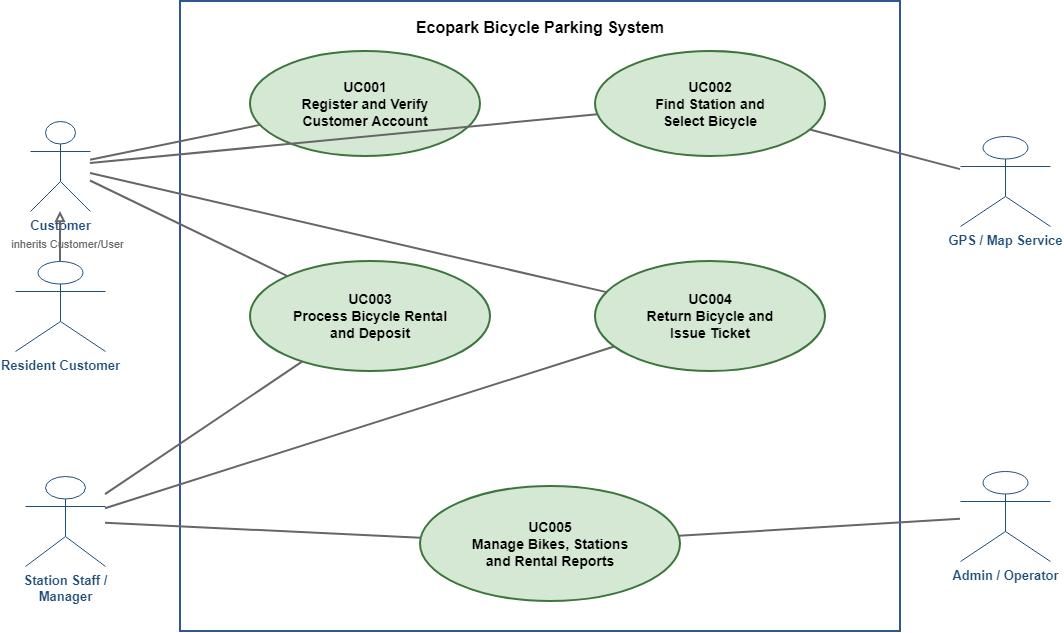
\includegraphics[width=\textwidth,height=0.82\textheight,keepaspectratio]{uc_overview.png}
\end{frame}

\begin{frame}{Implemented Scope: UC001--UC005}
\scriptsize
\begin{tabular}{p{0.12\textwidth}p{0.31\textwidth}p{0.47\textwidth}}
\toprule
\textbf{Use Case} & \textbf{Objective} & \textbf{Platform Outcome} \\
\midrule
UC001 & Customer accounts and verification & Registration and login; validation for name, phone number, ID document, and resident discount. \\
UC002 & Find stations and select bicycles & Live or manual GPS, distance and type filters, bicycle selection, request submission/cancellation, and handover geofence. \\
UC003 & Handover and deposit & Staff verify documents, collect a VND 200,000 deposit, retain documents, and mark the bicycle as rented. \\
UC004 & Return and ticket issuance & Cross-station return, fee calculation, resident discount, late surcharge, condition notes, and ticket summary. \\
UC005 & Operations management & Station and fleet CRUD, status reasons, report charts, audit logs, and CSV export. \\
\bottomrule
\end{tabular}
\end{frame}

\begin{frame}{EcoBike Deployment Architecture}
\centering
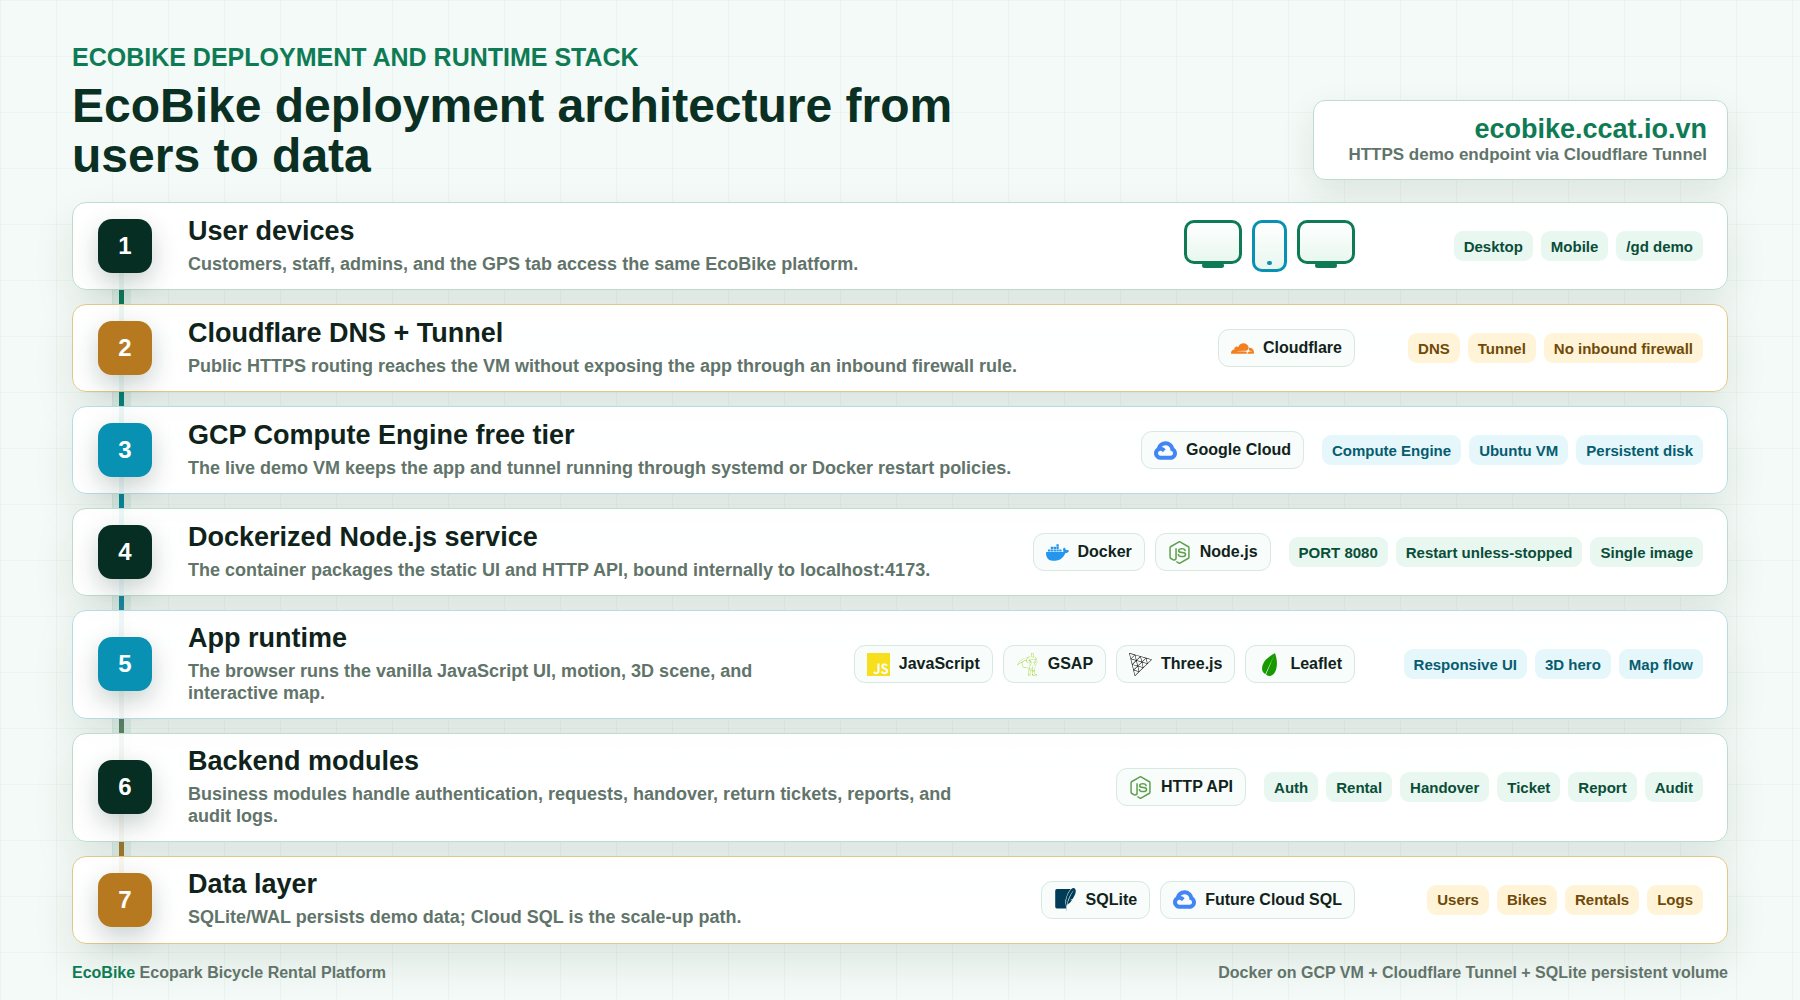
\includegraphics[width=\textwidth,height=0.86\textheight,keepaspectratio]{techstack/tech_stack_architecture_en.png}
\end{frame}

\begin{frame}{Data Design}
\centering
\resizebox{0.96\textwidth}{!}{%
\begin{tikzpicture}[
  domaincard/.style={draw=EbpGreen,thick,rounded corners=4pt,fill=SoftGreen,minimum width=3.25cm,minimum height=1.78cm,align=left,font=\scriptsize,inner sep=7pt},
  core/.style={draw=EbpTeal,very thick,rounded corners=4pt,fill=cyan!8,minimum width=3.55cm,minimum height=2.12cm,align=left,font=\scriptsize,inner sep=8pt},
  support/.style={draw=EbpAmber,thick,rounded corners=4pt,fill=yellow!10,minimum width=3.25cm,minimum height=1.48cm,align=left,font=\scriptsize,inner sep=7pt},
  arr/.style={-{Latex[length=2mm]},draw=Ink,line width=0.85pt}
]
\node[core] (rental) at (0,0) {
  \textbf{Rental transactions}\\[1mm]
  RENTAL\_REQUESTS\\
  RENTALS\\
  DEPOSITS\\
  TICKETS
};
\node[domaincard] (identity) at (-4.55,0) {
  \textbf{Users \& profiles}\\[1mm]
  USERS\\
  CUSTOMER\_PROFILES\\
  RESIDENT\_CARDS\\
  STAFF
};
\node[domaincard] (fleet) at (4.55,0) {
  \textbf{Stations \& fleet}\\[1mm]
  STATIONS\\
  BIKE\_TYPES\\
  BIKES\\
  BIKE\_STATUS\_LOGS
};
\node[support] (policy) at (0,2.35) {
  \textbf{Pricing policy}\\
  resident discount, late surcharge, deposit
};
\node[support] (ops) at (0,-2.35) {
  \textbf{Operations reporting}\\
  revenue, fleet status, audit trail
};
\draw[arr] (identity.east) -- (rental.west);
\draw[arr] (fleet.west) -- (rental.east);
\draw[arr] (policy.south) -- (rental.north);
\draw[arr] (rental.south) -- (ops.north);
\end{tikzpicture}
}
\vspace{0.2cm}
\small The detailed ERD is in the report; this slide shows only the core data relationships around the rental lifecycle.
\end{frame}

\begin{frame}{Bicycle Rental Lifecycle}
\centering
\resizebox{0.92\textwidth}{!}{%
\begin{tikzpicture}[
  state/.style={draw=EcoparkGreen,thick,rounded corners=2pt,fill=SoftGreen,minimum width=2.9cm,minimum height=0.92cm,align=center,font=\scriptsize},
  bad/.style={draw=EcoparkAmber,thick,rounded corners=2pt,fill=yellow!12,minimum width=2.9cm,minimum height=0.92cm,align=center,font=\scriptsize},
  arr/.style={-{Latex[length=2.2mm]},thick,draw=Ink}
]
\node[state] (available) {Bike available};
\node[state,right=0.95cm of available] (pending) {Request\\pending pickup};
\node[state,right=0.95cm of pending] (rented) {Rental\\in progress};
\node[state,right=0.95cm of rented] (ticket) {Ticket\\completed};
\node[bad,below=0.85cm of pending] (cancel) {Cancel / expired};
\node[bad,below=0.85cm of ticket] (broken) {Broken / review};
\draw[arr] (available) -- (pending);
\draw[arr] (pending) -- (rented);
\draw[arr] (rented) -- (ticket);
\draw[arr] (pending) -- (cancel);
\draw[arr] (cancel) -| (available);
\draw[arr] (ticket) -- (broken);
\end{tikzpicture}
}
\end{frame}

\begin{frame}{Customer Mobile Flow}
\begin{columns}[T,totalwidth=0.98\textwidth]
\begin{column}{0.31\textwidth}
\centering
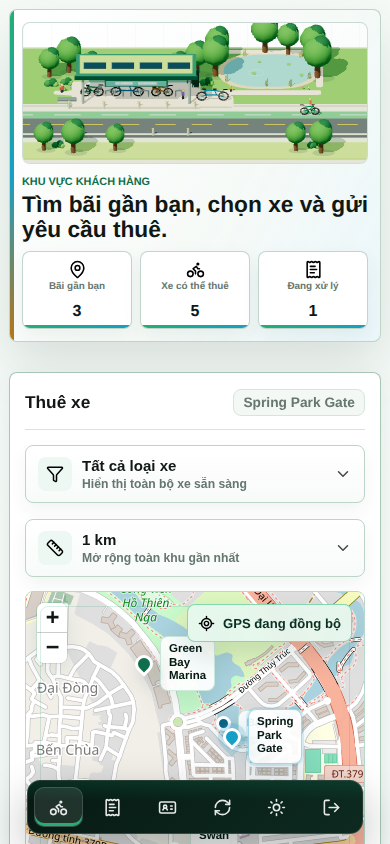
\includegraphics[width=\linewidth,height=0.62\textheight,keepaspectratio]{customer_mobile_overview.png}\\[1mm]
\slidecaption{Overview}
\end{column}
\begin{column}{0.31\textwidth}
\centering
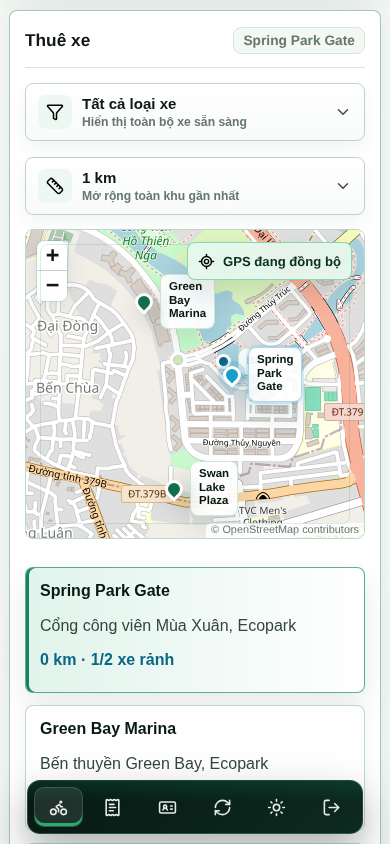
\includegraphics[width=\linewidth,height=0.62\textheight,keepaspectratio]{customer_mobile_search.png}\\[1mm]
\slidecaption{Find a station}
\end{column}
\begin{column}{0.31\textwidth}
\centering
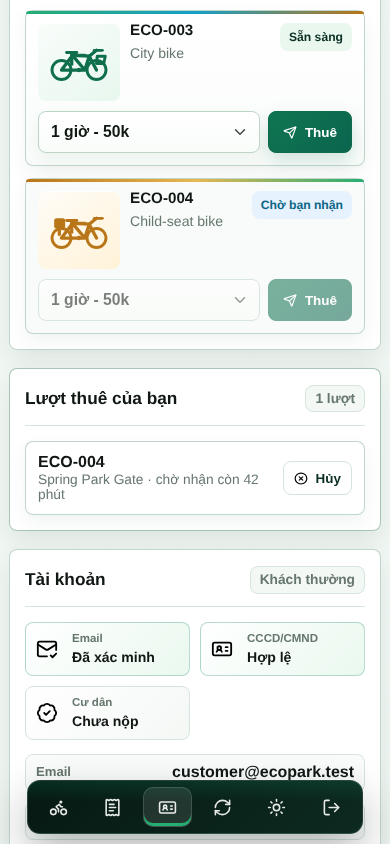
\includegraphics[width=\linewidth,height=0.62\textheight,keepaspectratio]{customer_mobile_bikes.png}\\[1mm]
\slidecaption{Select a bicycle}
\end{column}
\end{columns}
\vspace{0.15cm}
\scriptsize The mobile flow is split into unobstructed views above the bottom dock: overview, nearest-station results, and available-bicycle selection.
\end{frame}

\begin{frame}{Operations UI}
\begin{columns}[T,totalwidth=0.98\textwidth]
\begin{column}{0.49\textwidth}
\centering
\begin{minipage}[t][0.72\textheight][c]{\linewidth}
\centering
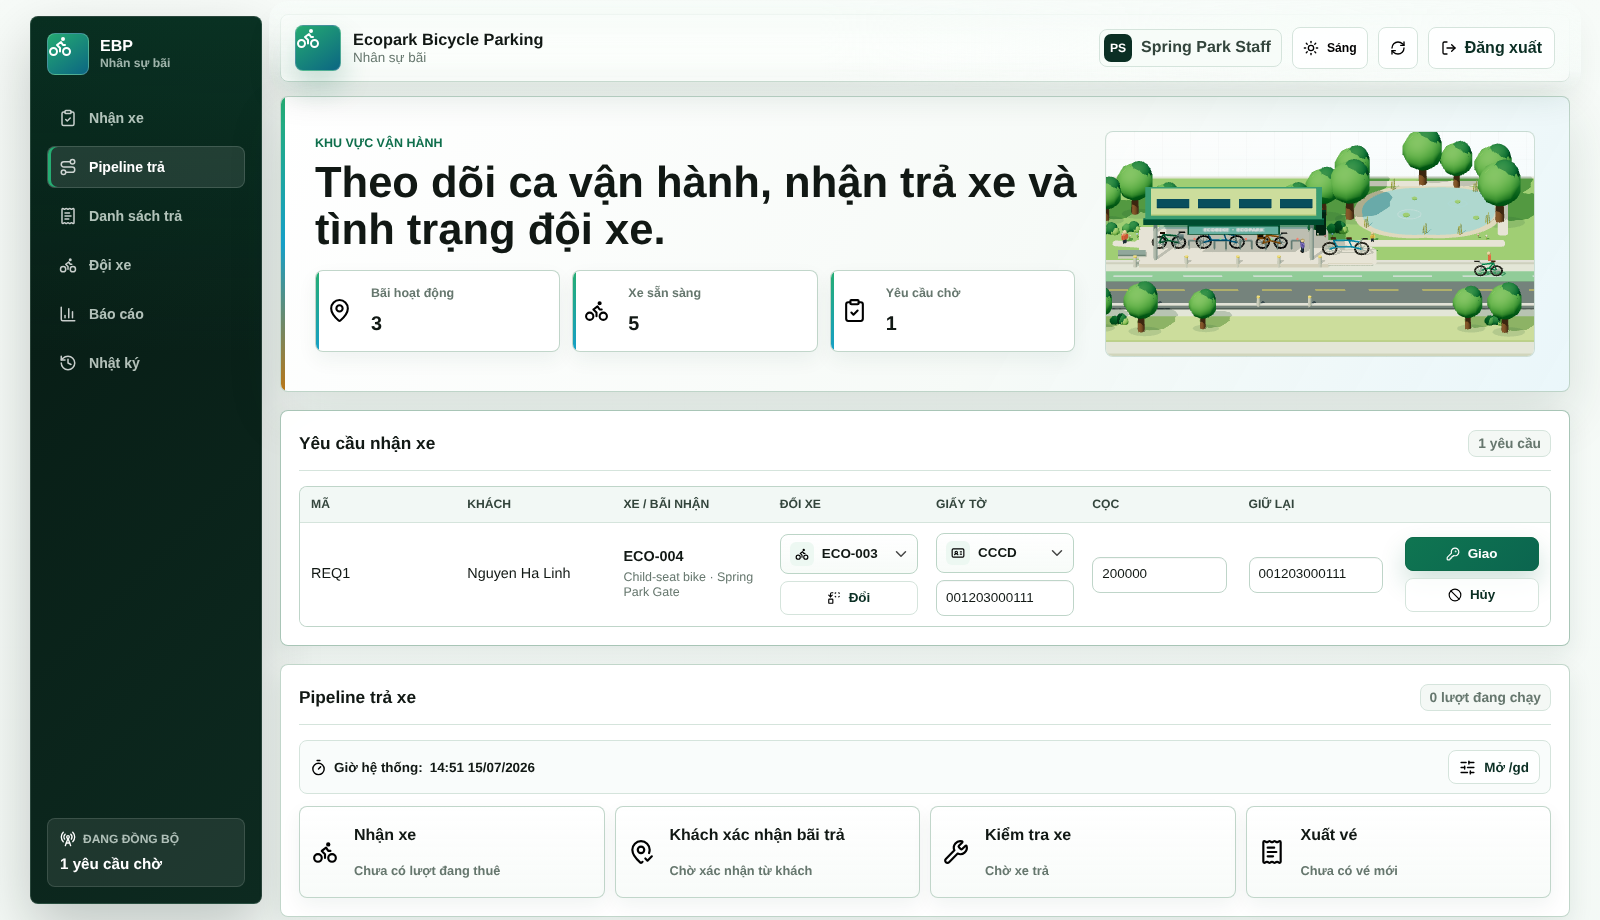
\includegraphics[width=\linewidth,height=0.70\textheight,keepaspectratio]{operations_overview.png}
\end{minipage}
\end{column}
\begin{column}{0.49\textwidth}
\centering
\begin{minipage}[t][0.72\textheight][c]{\linewidth}
\centering
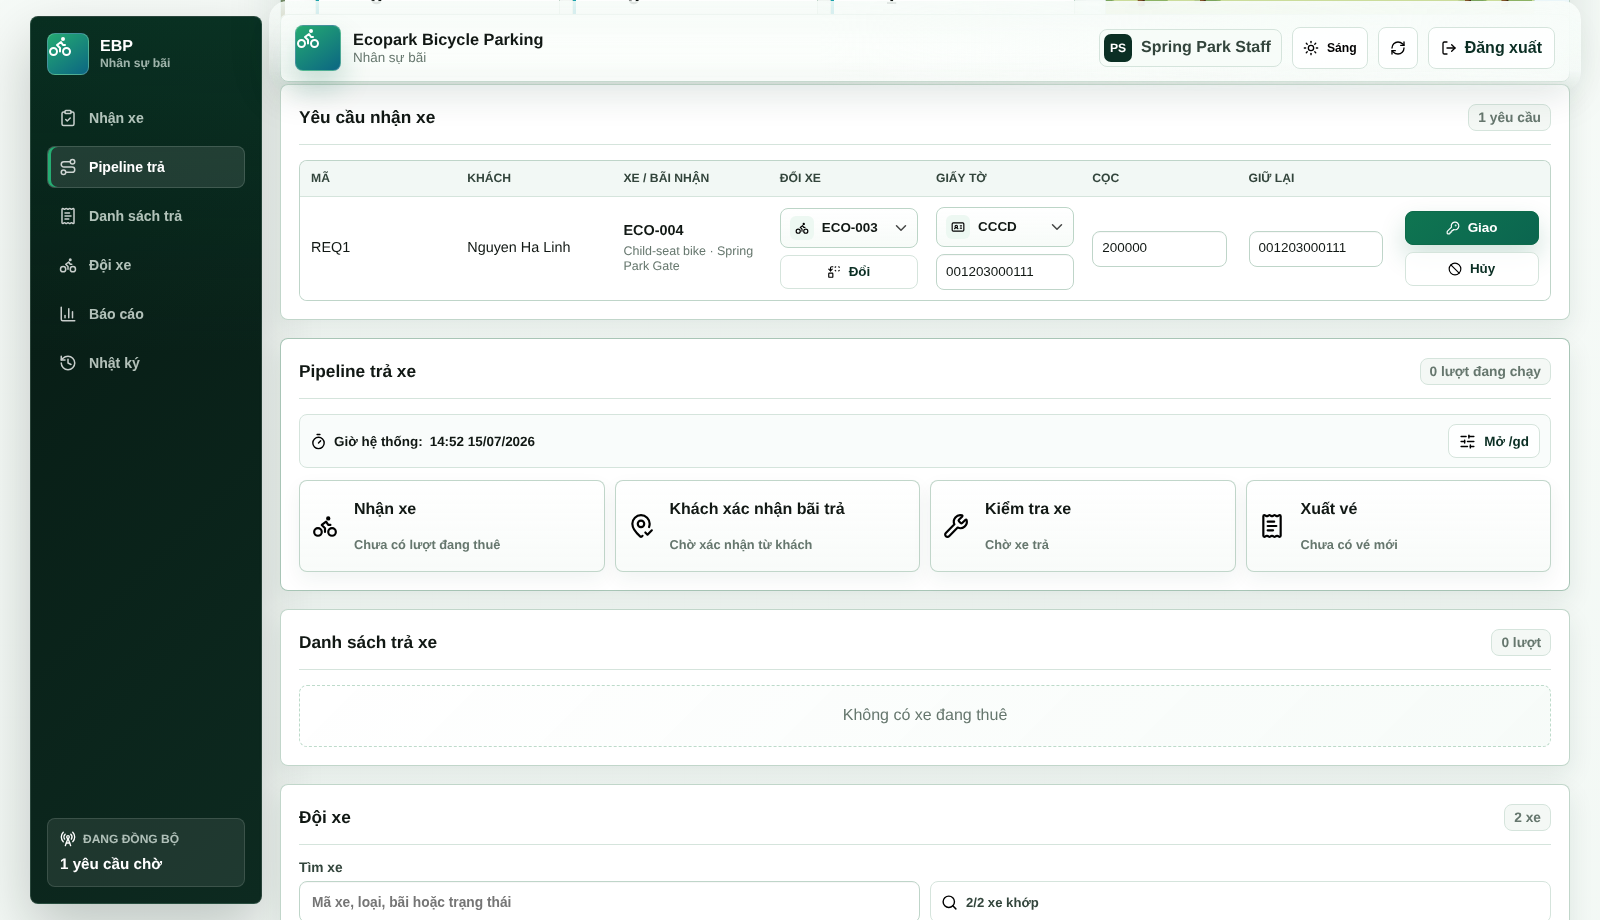
\includegraphics[width=\linewidth,height=0.70\textheight,keepaspectratio]{operations_pipeline.png}
\end{minipage}
\end{column}
\end{columns}
\vspace{-1mm}
\begin{columns}[T,totalwidth=0.98\textwidth]
\begin{column}{0.49\textwidth}
\centering
\slidecaption{Operations overview}
\end{column}
\begin{column}{0.49\textwidth}
\centering
\slidecaption{Pickup requests and return pipeline}
\end{column}
\end{columns}
\vspace{0.15cm}
\scriptsize Operations screenshots capture each state separately so the overview and processing areas remain clear during the presentation.
\end{frame}

\begin{frame}{Light/Dark Mode}
\begin{columns}[T,totalwidth=0.98\textwidth]
\begin{column}{0.58\textwidth}
\centering
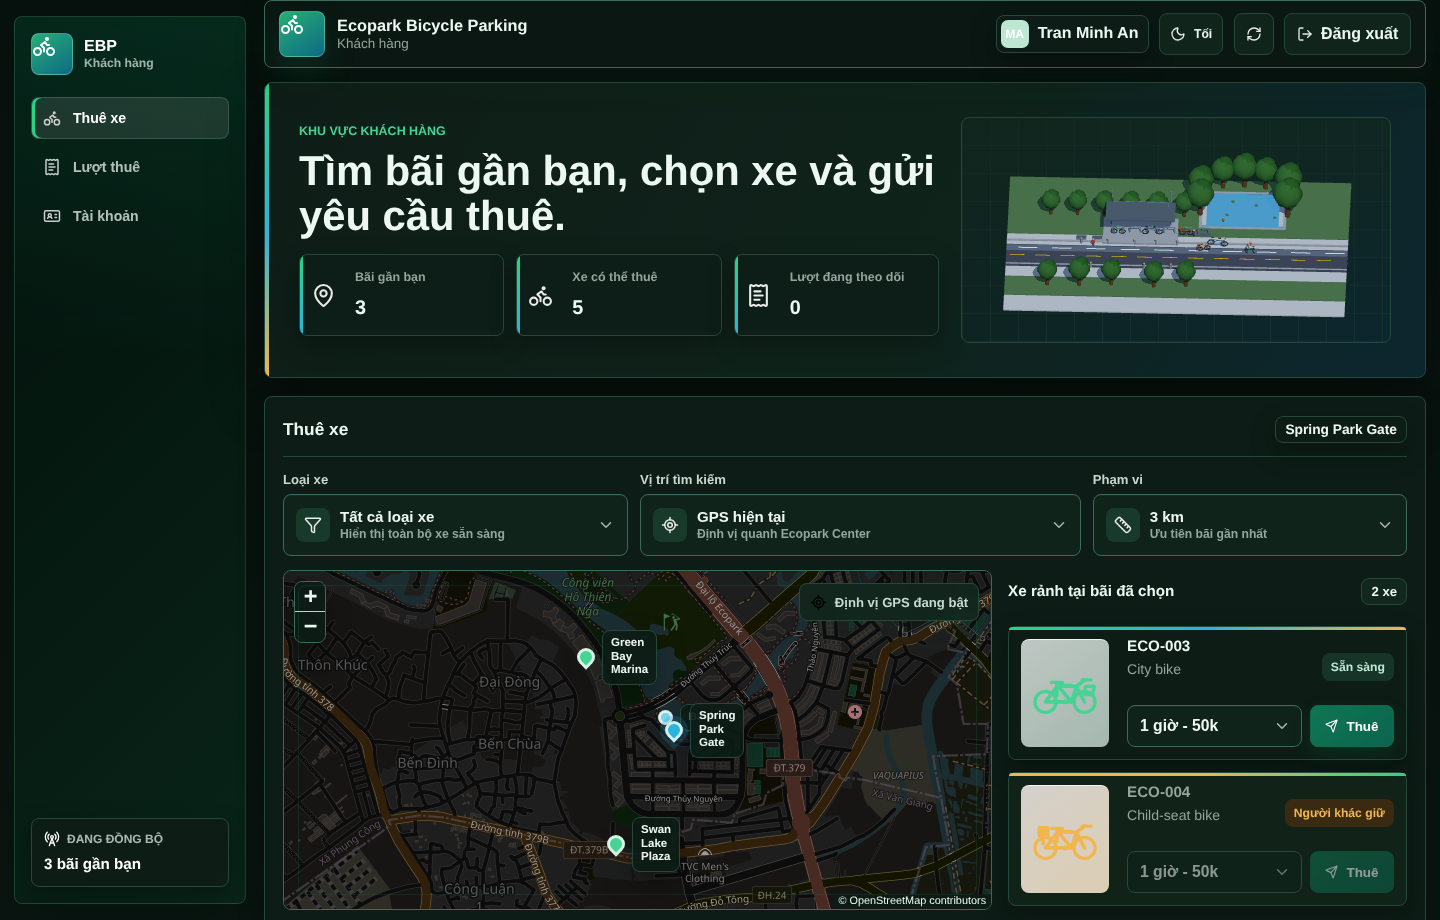
\includegraphics[width=\linewidth,height=0.72\textheight,keepaspectratio]{darkmode_customer.png}
\end{column}
\begin{column}{0.37\textwidth}
\small
\begin{itemize}\tightitems
  \item Light, dark, and system themes are persisted in the browser.
  \item The Leaflet map has a dedicated dark treatment that avoids a harsh white map surface.
  \item Account cards, dropdowns, charts, and forms share the same design tokens.
  \item The 3D scene preserves enough contrast to distinguish bicycles, roads, the lake, and trees.
\end{itemize}
\end{column}
\end{columns}
\end{frame}

\begin{frame}{Demo Director for Alternative Flows}
\begin{columns}[T,totalwidth=0.98\textwidth]
\begin{column}{0.61\textwidth}
\centering

\includegraphics[width=\linewidth,height=0.72\textheight,keepaspectratio]{gps_demo.png}
\end{column}
\begin{column}{0.34\textwidth}
\scriptsize
\begin{tikzpicture}[
  stepcard/.style={draw=EbpBorder,rounded corners=3pt,fill=white,text width=0.95\linewidth,minimum height=1.05cm,align=left,inner sep=6pt}
]
\node[stepcard] at (0,0) {\textbf{1. Select a user / session}\\Find a customer account and select its session when available.};
\node[stepcard] at (0,-1.35) {\textbf{2. Move the user's GPS}\\Stream the route polyline to the customer map.};
\node[stepcard] at (0,-2.70) {\textbf{3. Fast-forward system time}\\Demonstrate expiration and late surcharges.};
\node[stepcard] at (0,-4.05) {\textbf{4. Validate the station radius}\\Requests may be created anywhere; handover and return require proximity.};
\end{tikzpicture}
\end{column}
\end{columns}
\end{frame}

\begin{frame}{API and Backend Implementation}
\scriptsize
\begin{tabular}{p{0.24\textwidth}p{0.20\textwidth}p{0.46\textwidth}}
\toprule
\textbf{API Group} & \textbf{Role} & \textbf{Main Endpoints} \\
\midrule
Auth/Profile & Public/Customer & \texttt{/api/auth/register}, \texttt{/api/auth/login}, \texttt{/api/customer/resident-card}. \\
Station/Bike & Customer & \texttt{/api/stations}, \texttt{/api/stations/:id/bikes}, \texttt{/api/rental-requests}. \\
Handover/Return & Staff/Admin & \texttt{/api/staff/pending-requests}, \texttt{/api/staff/handover}, \texttt{/api/staff/return}. \\
Admin/Report & Staff/Admin & \texttt{/api/admin/bikes}, \texttt{/api/admin/reports}, \texttt{/api/admin/bike-status-logs}. \\
\bottomrule
\end{tabular}
\vspace{0.25cm}
\begin{itemize}\tightitems
  \item Server-side validation covers names, phone numbers, ID documents, and duplicate data.
  \item Rental, handover, and return operations use transactions to prevent double-booking.
  \item Audit logs record bicycle status changes together with the operator, station, and reason.
\end{itemize}
\end{frame}

\begin{frame}{Reporting Dashboard}
\begin{columns}[T,totalwidth=0.98\textwidth]
\begin{column}{0.58\textwidth}
\centering
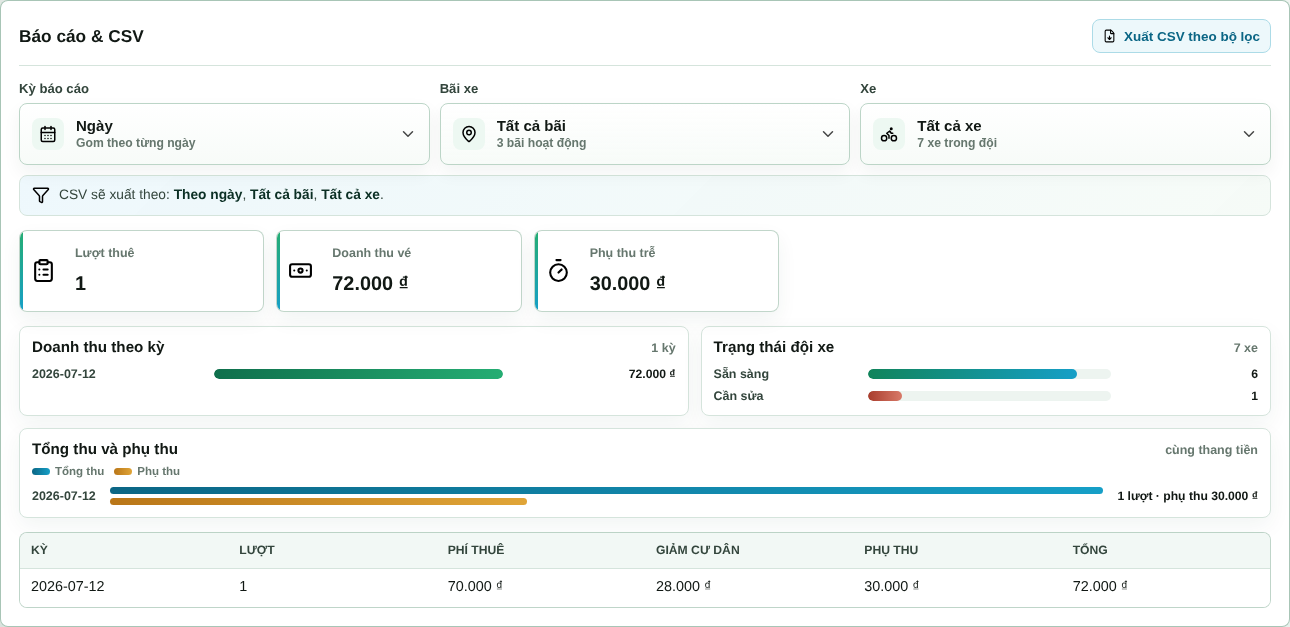
\includegraphics[width=\linewidth,height=0.72\textheight,keepaspectratio]{operations_report.png}
\end{column}
\begin{column}{0.37\textwidth}
\small
\begin{itemize}\tightitems
  \item Revenue charts use a consistent monetary scale across reporting periods.
  \item Fleet status distinguishes available, rented, and maintenance-required bicycles.
  \item Rental counts and late surcharges appear alongside the underlying report table.
  \item CSV exports preserve the filters currently selected on the dashboard.
  \item Audit logs identify who changed each bicycle's status and why.
\end{itemize}
\end{column}
\end{columns}
\end{frame}

\begin{frame}{Testing and Evidence}
\centering
\begin{tikzpicture}[
  card/.style={draw=EbpBorder,rounded corners=3pt,fill=white,minimum width=3.10cm,minimum height=1.66cm,align=left,inner xsep=6pt,inner ysep=5pt}
]
\node[card] (api) at (-5.05,1.82) {
  \begin{minipage}[t][1.22cm][t]{2.62cm}\raggedright
  {\large\bfseries\color{EbpGreen}24/24}\\[0.2mm]
  {\scriptsize\bfseries Backend API tests}\\[0.1mm]
  {\tiny Station staff + rental flow}
  \end{minipage}
};
\node[card] (ui) at (-1.68,1.82) {
  \begin{minipage}[t][1.22cm][t]{2.62cm}\raggedright
  {\large\bfseries\color{EbpTeal}5}\\[0.2mm]
  {\scriptsize\bfseries UI viewports}\\[0.1mm]
  {\tiny Customer, staff, admin}
  \end{minipage}
};
\node[card] (uc) at (1.68,1.82) {
  \begin{minipage}[t][1.22cm][t]{2.62cm}\raggedright
  {\large\bfseries\color{EbpAmber}UC}\\[0.2mm]
  {\scriptsize\bfseries End-to-end smoke}\\[0.1mm]
  {\tiny /gd, handover, return, CSV}
  \end{minipage}
};
\node[card] (ci) at (5.05,1.82) {
  \begin{minipage}[t][1.22cm][t]{2.62cm}\raggedright
  {\large\bfseries\color{EbpGreen}CI/CD}\\[0.2mm]
  {\scriptsize\bfseries GitHub Actions}\\[0.1mm]
  {\tiny Check, coverage, smoke, Docker}
  \end{minipage}
};
\node[card] (line) at (-3.37,-0.10) {
  \begin{minipage}[t][1.22cm][t]{2.62cm}\raggedright
  {\large\bfseries\color{EbpGreen}80.67\%}\\[0.2mm]
  {\scriptsize\bfseries Line coverage}\\[0.1mm]
  {\tiny Node.js built-in coverage}
  \end{minipage}
};
\node[card] (branch) at (0,-0.10) {
  \begin{minipage}[t][1.22cm][t]{2.62cm}\raggedright
  {\large\bfseries\color{EbpTeal}71.46\%}\\[0.2mm]
  {\scriptsize\bfseries Branch coverage}\\[0.1mm]
  {\tiny Node.js built-in coverage}
  \end{minipage}
};
\node[card] (function) at (3.37,-0.10) {
  \begin{minipage}[t][1.22cm][t]{2.62cm}\raggedright
  {\large\bfseries\color{EbpAmber}84.92\%}\\[0.2mm]
  {\scriptsize\bfseries Function coverage}\\[0.1mm]
  {\tiny Node.js built-in coverage}
  \end{minipage}
};
\end{tikzpicture}
\vspace{0.16cm}
\begin{center}
\begin{tikzpicture}
\node[draw=EbpBorder,rounded corners=3pt,fill=SoftGreen,text width=0.88\textwidth,inner sep=7pt,align=left] {
  \scriptsize\textbf{Test scenario:} open /gd, select the correct user, verify that the customer marker follows the GPS stream, submit a rental request, complete staff handover, confirm a return station within the valid radius, issue the ticket, and inspect the dashboard, CSV export, and audit log.
};
\end{tikzpicture}
\end{center}
\end{frame}

\begin{frame}{Open the Live Demo}
\begin{columns}[T,totalwidth=0.96\textwidth]
\begin{column}{0.52\textwidth}
\centering

\includegraphics[width=\linewidth,height=0.68\textheight,keepaspectratio]{gps_demo.png}
\end{column}
\begin{column}{0.42\textwidth}
\small
\begin{enumerate}\tightitems
  \item Open the Customer, Staff/Admin, and \texttt{/gd} tabs.
  \item Submit a customer request, then use \texttt{/gd} to move the user into pickup range before handover.
  \item Staff verify documents, collect the VND 200,000 deposit, and hand over the bicycle.
  \item The customer confirms the return station; staff issue the ticket and review any surcharge.
  \item Finish with the dashboard, audit log, and CSV export.
\end{enumerate}
\vspace{0.2cm}
{\scriptsize\bfseries\color{EbpGreen}Live demo: complete all five steps in the app.}
\end{column}
\end{columns}
\end{frame}

\end{document}
